\chapter{Current Practice}
Three copies of the dissertation (1 original and 2 copies, either xerographic, photocopied, offset or letter quality printer) are to be supplied to the Library. In addition, an abstract independent of the document is to be supplied to the Library. The announcement for Ph.D. dissertation defense is to be given to The Office of the Registrar at least 1½ weeks prior to the defense. A sample defense announcement can be found in sample pages.

You must hand in your dissertation in person to Doris Oliver. If Doris is not available, Nydia Cruz can also accept dissertations. Dissertations cannot be mailed to the Library and cannot be handed in by another person.

Doris Oliver is available to accept dissertations from 9:30am - 1:00pm and 2:00pm - 4:00 pm, M-F. Appointments are not necessary but are highly recommended.

\subsection*\normalsize\emph{Publication Agreement and Survey Forms}

The UMI Publication Agreement Form and a Survey of Earned Doctorates Form are submitted with the dissertation. The forms are available from Doris Oliver and online. Both forms must be completed and returned to Doris Oliver with the final dissertation. The UMI Publication Agreement Form includes the application form. This should be read, filled out and returned to Doris Oliver. The Survey of Earned Doctorates form is available online in two documents: the Survey of Earned Doctorates brochure and the Survey of Earned Doctorates form online.  UMI also provides a brochure on privacy as it relates to dissertations.

\subsection*\normalsize\emph{Use of Previously Published work in your dissertation}

If you are including previously published material as part of your dissertation, either as an appendix or as part of the body of your paper, you must obtain written permission from the publisher to have the work included as part of your paper.   Even if you are the author of the published material, you still must get permission from the publisher.    

Please view the dissertation specifications on the library website for information about UMI/Proquest's guide to copyright and copyright infringement. 

UMI/Proquest also includes information written by Kenneth Crews, a professor at Indiana University on the issue of copyright.  His work covers how to request permission from publishers, and sample permission letters.

\Large It is the responsibility of the student to ensure that all portions of their dissertation adhere to copyright law.  


\normalsize 

\begin{figure}[htp]
\centering
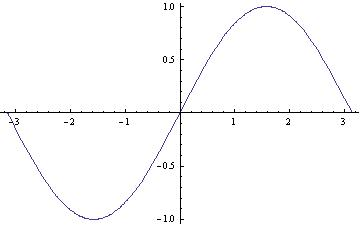
\includegraphics{sin_x.jpg}
\caption{Transverse momentum distributions}\label{fig:erptsqfit}
\end{figure}

